\section{Simulations et tests d'intégration}

\subsection{Les tests d'intégration}

Il s'agit dans la sous-section suivante de présenter les différents tests d'intégrations.
La liste à puce ci-dessous présente les divers tests avec une brève présentation, les éléments validant la bonne intégration de l'IP.
Pour chacune de ces étapes, les outils Xilinx Vivado et Xilinx SDK seront employés.

\begin{itemize}
	\item Dans un cas de couplage direct, le CPU effectue des cycles d'écriture et de lecture pour chaque registre de l'IP.
	Afin de valider la bonne intégration, un ILA est placé sur l'interface AXI4-Lite pour observer les signaux (VALID,READY) et les bus (ADDR,DATA) de chaque canal (canal d'écriture et canal de lecture).
	\item Dans une cas de couplage indirect, l'IP doit également coopérer avec le DMA afin de transférer des données de l'IP vers les mémoires vives.
	Les éléments de validation sont les mêmes que le point précédent.
	\item Les lignes d'interruptions de chaque bloc sont testées une à une.
	Celles-ci sont set à l'aide du CPU (par écriture à l'adresse correspondante) au niveau logique 0 (actives à l'état bas).
	Pour valider la bonne intégration de l'IP dans le SoC, il s'agit de placer un ILA sur les lignes d'interruptions de chaque IP et la ligne d'interruption nIT\_CPU.
	Une table d'adresse de branchement sera définie arbitrairement et configurée dans l'IP.
	Il est important de valider la bonne lecture de l'adresse de branchement de la part du CPU, en plaçant également un ILA sur l'interface AXI4-Lite.
	Des breakpoints sur Xilinx SDK seront utiles pour vérifier si le CPU arrête bien son exécution et branche sur la bonne sous-routine d'interruption.
	\item Pour finir, des tests simultanés sont effectués avec les IT des diverses IP sous plusieurs configuration (niveau de priorité différent, masquage ou non etc).
	Les éléments de validation sont les mêmes que le point précédent.
	L'exemple suivant éclairera ce propos. 
	
\end{itemize}

Par exemple, il existe deux configurations possibles (priorité et masquage) pour l'ensemble des 15 interruptions.
Le triplet (IT,priorité,masquage) offre $15\times8\times2$ soit $240$ combinaisons possibles comme le présente la figure ci-dessous.

\begin{figure}[h!]
	\centering
	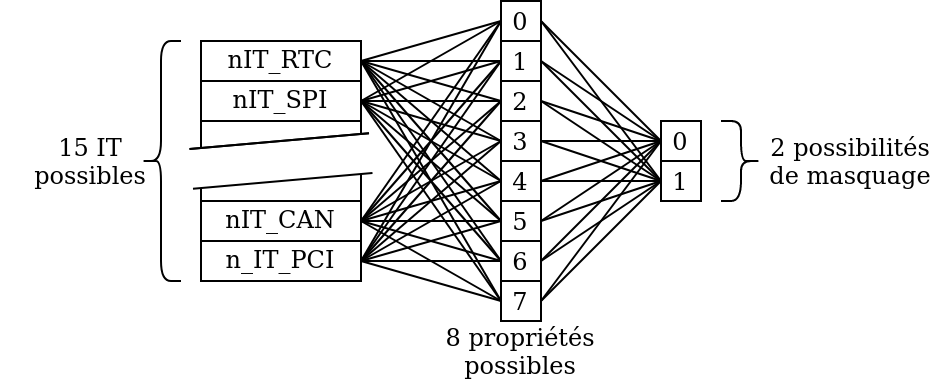
\includegraphics[width=0.7\linewidth]{figure/combinaisons_integration.png}
	\caption{Exemple de couverture de tests d'intégrations}
	\label{fig:combinaisons_integration}
\end{figure}

Il s'agit de couvrir l'ensemble des 240 triplets possibles tout en vérifiant que les priorités des interruptions soient respectées. Pour se faire, 14 IT ont une priorité fixes et seulement 1 varie selon le niveau de priorité et le masquage.

\subsection{Étapes non nécessaires}

À ce stade du développement de l'IP, certaines étapes étudiées ne sont pas nécessaires.

\begin{itemize}
	\item Par exemple, les étapes de modélisation et de vérification au niveau système réalisable sur SystemC.
	Il n'y a aucun profit à tirer de cet outil car l'IP est déjà décrite et la spécification et conception au niveau système ont déjà été pensées.
	\item En ce qui concerne l'outil de codesign Cofluent étudié en travaux pratiques, celui-ci est utile en amont de la conception.
	Cofluent permet de réaliser des études de faisabilité, déterminer des propriétés pour un circuit donné et effectuer du design exploration.
\end{itemize}


